\subsection{Systemarchitektur}

Dieses Kapitel beschreibt die Komponenten des cloudbasierten Praxisrufsystems und wie diese erweitert werden.
Abbildung 7.1 gibt einen Überblick über die Systemkomponenten und welche Module diese beinhalten.
Dabei sind Module, die im Rahmen dieses Projektes entwickelt oder neu integriert werden, grün umrandet.
Die Pfeile zwischen Modulen zeigen gerichtete Abfragen und Aufrufe zwischen den Komponenten.
Alle Abfragen zwischen Services sowie zwischen Modulen des Cloudservices finden über die API Schnittstellen der jeweiligen Module statt.

\begin{figure}[h]
    \centering
    \begin{minipage}[b]{0.8\textwidth}
        \fbox{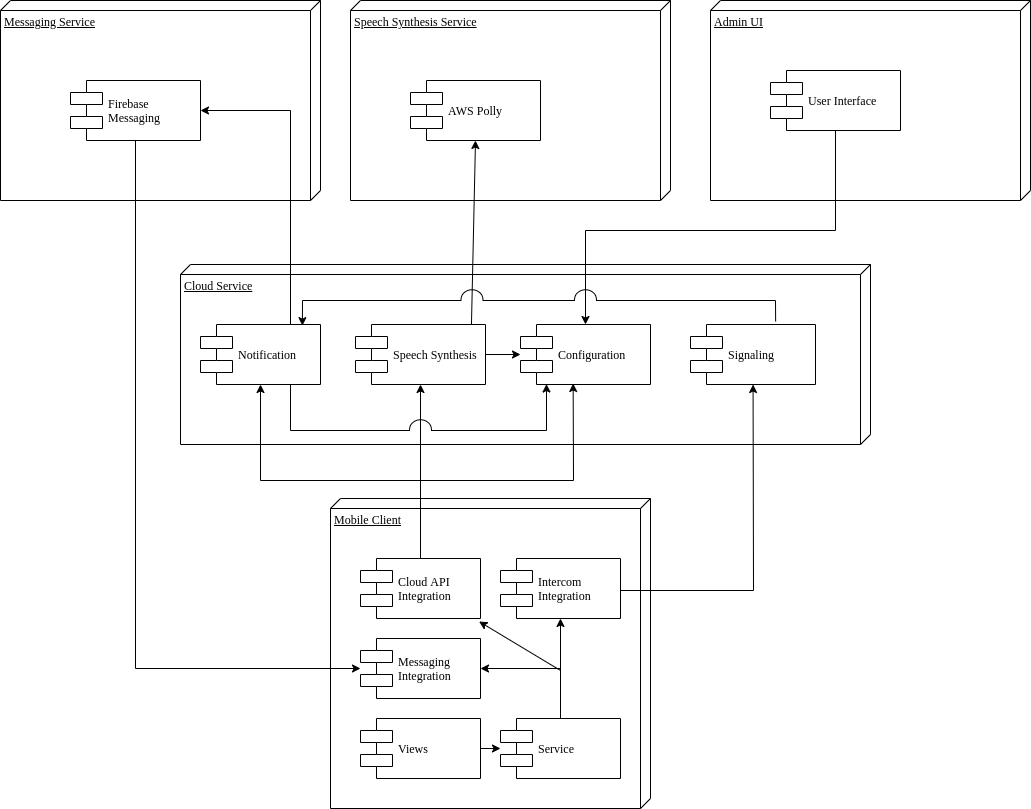
\includegraphics[width=\textwidth]{graphics/diagramms/Component_System_V03}}
        \caption{Systemkomponenten}
    \end{minipage}
\end{figure}

\subsubsection{Systemkomponenten}

Dieses Kapitel beschreibt die in Abbildung 7.1 abgebildeten Systemkomponenten.
Dabei wird für jede Komponente beschrieben, welche Aufgaben ihr zufallen und wie sie im Rahmen dieses Projektes erweitert wird.

\textbf{Cloudservice}

Der Cloudservice bildet die zentrale Serverkomponente von Praxisruf.
Zu Beginn dieses Projektes umfasst der Cloudservice die beiden Domänen Notification und Configuration.
Dabei ist die Domäne Notification für das Versenden von Benachrichtigungen und die Domäne Configuration für die Verwaltung und Auswertung der Konfigurationen verantwortlich.
Die relevanten Empfänger für eine Benachrichtigung werden in der Configuration Domain ermittelt.
Um auf diese Informationen zugreifen zu können, muss aus der Domäne Notification eine Abfrage an die Domäne Configuration gesendet werden.
Die Configuration-Domäne bietet dazu eine HTTP Schnittstelle~\cite{ip5}.

Die Trennung der Domänen wurde im Vorgängerprojekt lediglich auf Package-Ebene realisiert.
Mit diesem Projekt soll die Trennung einen Schritt weiter gehen.
Der Cloudservice wird in Module aufgeteilt.
Diese Module werden weiterhin in einer einzelnen Applikation zusammengefasst, können aber zu einem späteren Zeitpunkt in einzelne Microservices betrieben werden.

Nachdem die Auftrennung der bestehenden Domänen in Module stattgefunden hat, wird der Cloudservice erweitert.
Es werden die zwei Module Signaling und Speech Synthesis umgesetzt.
Das neue Modul Signaling ist für die Signalvermittlung zwischen Mobile Clients verantwortlich.
Es übernimmt die Aufgabe der Signaling Instanz für den Aufbau von Sprachverbindungen mit WebRTC.
Das Modul Signaling hat eine funktionale Abhängigkeit zum Modul Notification.
Es verwendet die API des Notification Moduls, um Empfänger mit Benachrichtigungen über verpasste Verbindungen zu informieren.

Das neue Modul Speech Synthesis dient als Schnittstelle zu einem externen Provider für Sprachsynthese.
Dies ermöglicht es, die Sprachsynthese als Teil der API des Cloudservice anzubieten.
Dadurch können Clients aller Plattformen und auch Systeme, die künftig angebunden werden, auf die Sprachsynthese zugreifen.
Weil alle Clients die Daten aus derselben Schnittstelle beziehen, ist garantiert, dass die Konfiguration und Funktionsweise dieselbe für alle Clients ist.

\textbf{Mobile Client}

Der Mobile Client ist eine mobile Appliaktion, über welche Praxisruf bedient werden kann.
Der mit dem Vorgängerprojekt umgesetzte Mobile Client erlaubt es Benachrichtigungen zu versenden und empfangen~\cite{ip5}.
Dieser Mobile Client wird durch eine native iOS Applikation ersetzt.
Dabei wird sämtliche Funktionen des Mobile Clients aus dem Vorgängerprojekt in die native App migriert.
Weiter werden die Funktionen Gegensprechanlage und Sprachsynthese für empfangene Benachrichtigungen umgesetzt.

\textbf{Admin UI}

Das Admin UI ist eine Webapplikation, über welche die Konfiguration des Praxisrufsystems verwaltet werden kann.
Die Konfiguration des Systems wird für Gegensprechanlage und Sprachsynthese erweitert.
Für die Gegensprechanlage müssen Buttons konfiguriert werden können.
Diese beinhalten Anzeigetext und Teilnehmer einer Sprachverbindung.
Weiter muss pro Benachrichtigung konfigurierbar sein, ob ihr Inhalt bei Empfang vorgelesen werden sollen.
Das Admin UI muss erweitert werden, um die Verwaltung der erweiterten Konfiguration zu ermöglichen.

\textbf{Messaging Service}

Der Messaging Service ist für die Zustellung von Push Benachrichtigungen an Mobile Clients verantwortlich.
Der Cloudservice muss an den Messaging Service angebunden sein, um Benachrichtigungen anhand der Konfiguration zu versenden~\cite{ip5}.
Die Anbindung des Cloudservices an den Messaging Service ist mit dem Vorgängerprojekt bereits umgesetzt und muss für dieses Projekt nicht angepasst werden.
Die neu entwickelte native iOS App muss hingegen an den Messaging Service angebunden werden, um Benachrichtigungen zu empfangen.
Als Messaging Service wird Firebase Cloud Messaging verwendet.

\clearpage

\textbf{Speech Synthesis Service}

Um Sprachsynthese zu ermöglichen, wird ein externer Service angebunden.
Dieser übernimmt die Konvertierung von Text aus Benachrichtigungen zu Sprachdaten.
Die Anbindung an den Speech Synthesis Service wird ausschliesslich im Cloudservice implementiert.
Sämtliche andere Komponenten die Sprachdaten benötigen, fragen diese beim Cloudservice ab.
Die REST API des Cloudservice wird um entsprechende Endpunkte erweitert.
Als Speech Synthesis Service wird Amazon Polly verwendet.

\subsubsection{Modularisierung Cloudservice}

Der mit dem Vorgängerprojekt umgesetzte Cloudservice ist als monolithische Applikation implementiert.
Er trennt intern die beiden Domänen Notification und Configuration.
Die Domäne Configuration ist für die Verwaltung und Auswertung der Konfiguration des Systems und die Domäne Notification für das Versenden von Benachrichtigungen verantwortlich.
Abhängigkeiten zwischen den beiden Domänen ist über eine REST-Schnittstelle abstrahiert.

Die Trennung der Domänen, erlaubt es die Anwendung zukünftig in mehrere Microservices aufzuteilen.
Diese könnten unabhängig betrieben und erweitert werden.
Weiter wird es dadurch möglich, einzelnen Teilen der Applikation mehr Ressourcen zuzuteilen.
Die Trennung der Domänen in eigene Microservices wurde im Rahmen des Vorgängerprojektes noch nicht vorgenommen.
Die beiden Domänen wurden lediglich durch die Package Struktur innerhalb eines einzelnen monolithischen Services getrennt.

Mit diesem Projekt wir die Trennung der Domänen innerhalb des Cloudservice verstärkt.
Die Applikation wird in strikt getrennte Module aufgeteilt.
Dabei wird pro Domäne ein Modul erstellt.
Dieses kapselt sämtliche Domänenobjekte, Services und Schnittstellen der jeweiligen Domäne.
Dadurch ist garantiert, dass die Domänen sauber voneinander getrennt sind.
Sämtliche Kommunikation zwischen den Modulen muss über die API der jeweiligen Module geschehen.

Es werden die vier Domänen-Module Configuration, Notification, Spech Synthesis und Signaling definiert.
Das Modul Configuration beinhaltet alle Domänenobjekte, Services und Schnittstellen für die Verwaltung, Auswertung und Abfrage der Systemkonfiguration.
Das Modul Notification beinhaltet alle Domänenobjekte, Services und Schnittstellen für das Versenden von Benachrichtiungen.
Das Modul Speech Synthesis beinhaltet die Anbindung an den Speech Synthesis Service.
Es stellt eine Schnittstelle zur Verfügung, über die Sprachdaten angefragt werden können.
Das Modul Signaling dient als Signaling Instanz für den Aufbau von Sprachverbindungen mit WebRTC\@.
Es beinhaltet Domänenobjekte, Services und Schnittstellen für die Signalvermittlung zwischen Mobile Clients.

Weiter werden die zwei Module Commons und App definiert.
Komponenten, welche in mehr als einer Domäne verwendet werden, werden in ein zusätzliches Commons Modul verlegt.
Dazu gehören Data Transfer Objects für Schnittstellen zwischen den Modulen, geteilte Clients um Abfragen auf andere Module abzusetzen sowie Komponenten Fehlerhandling.
Das Modul App hat eine Abhängigkeit auf alle Domänen Module und bietet ein Modul, über welches diese als einzelne Applikation gestartet werden können.
Das Modul beinhaltet weiter die globale Security Konfiguration des Systems.
Dadurch kann sichergestellt werden, dass diese für alle Systemteile angewendet wird.

Der Cloudservice wird weiterhin als monolithische Applikation betrieben.
Die Modularisierung garantiert dabei eine strikte Trennung der Domänen.
In Zukunft können einzelne Module aus dem Cloudservice ausgelöst und als eigenständige Applikationen betrieben werden.

\clearpage

\subsubsection{Domänenmodell Cloudservice}

Das Domänenmodell Cloudservices wird für die Integration von Sprachsynthese und Gegensprechanlage erweitert.
Abbildung 7.2 zeigt das vollständige Domänenmodell der Domänen Configuration und Notification.
Dabei sind Felder und Entitäten die in diesem Projekt hinzugefügt werden grün markiert.
Die neuen Domänen Speech Synthesis und Signaling führen keine persistenten Daten.
Die Services und Komponenten dieser Domänen sind in den Kapiteln 7.3 und 7.4 beschrieben.

\begin{figure}[h]
    \centering
    \begin{minipage}[b]{0.9\textwidth}
        \fbox{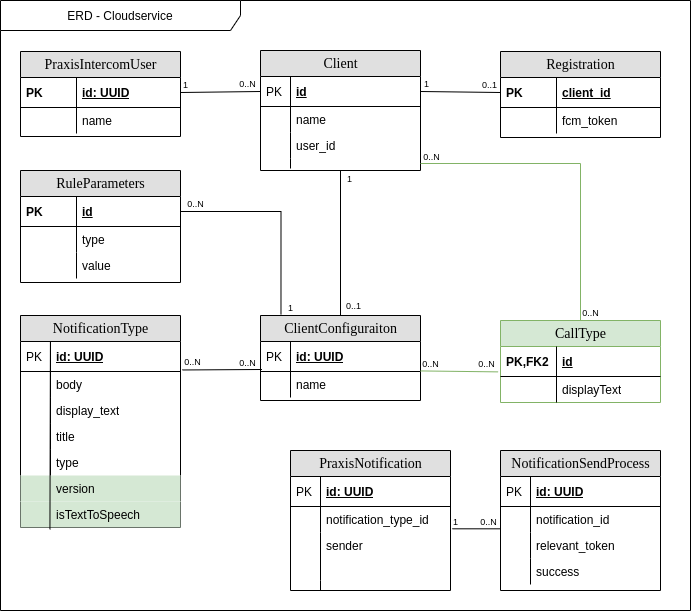
\includegraphics[width=\textwidth]{graphics/diagramms/erd_v02}}
        \caption{Entitiy Relationship Diagramm - Cloudservice}
    \end{minipage}
\end{figure}

\clearpage
